\documentclass{standalone}       % What kind of document this is
\usepackage{tikz}             % Import the tikz package
\usetikzlibrary{automata}     % Import library for drawing automata
\usetikzlibrary{positioning}  %                 ...positioning nodes
\usetikzlibrary{arrows}       %                 ...customizing arrows
\tikzset{node distance=2.5cm, % Minimum distance between two nodes. Change if necessary.
    every state/.style={      % Sets the properties for each state
        semithick,
        fill=gray!10},
    initial text={},          % No label on start arrow
    double distance=2pt,      % Adjust appearance of accept states
    every edge/.style={       % Sets the properties for each transition
    draw,
    ->,>=stealth',            % Makes edges directed with bold arrowheads
    auto,
    semithick}}
\let\epsilon\varepsilon

\begin{document}
    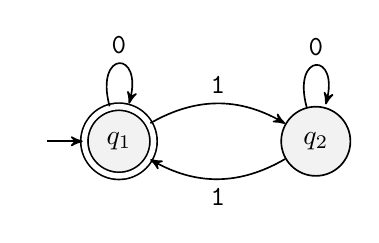
\begin{tikzpicture}
        \node[state, initial, accepting] (q1) {$q_1$};
        \node[state, right of=q1] (q2) {$q_2$};
        
        \draw (q1) edge[loop above] node {\tt 0} (q1);
        \draw (q1) edge[bend left] node {\tt 1} (q2);
        \draw (q2) edge[loop above] node {\tt 0} (q2);
        \draw (q2) edge[bend left] node {\tt 1} (q1);
    \end{tikzpicture}
\end{document}
